\documentclass[11pt]{article}
\usepackage[margin=1in]{geometry}
\usepackage{amsmath,amssymb,amsthm}
\usepackage[hidelinks]{hyperref}
\usepackage{enumitem}
\usepackage{graphicx}

\newtheorem{theorem}{Theorem}
\newtheorem{lemma}{Lemma}
\newtheorem{corollary}{Corollary}

\DeclareMathOperator{\spanop}{span}
\newcommand{\N}{\mathbb N}
\newcommand{\R}{\mathbb R}
\newcommand{\cU}{\mathcal U}
\newcommand{\one}{\mathbf 1}

\title{The Free Locally Convex Space on \(\mathbb N\cup\{p\}\) is Nuclear Exactly for Rapid \(P\)-Points}
\author{Agent lane 17}
\date{2026-06-20}

\begin{document}
\maketitle

\section*{Status}

This packet gives a claimed full answer to Problem 5.5 of Leiderman--Uspenskij
\cite{LU}: if \(p\in\beta\N\setminus\N\) and \(X=\N\cup\{p\}\), then
\[
   L(X)\text{ is nuclear}
   \quad\Longleftrightarrow\quad
   L(X)\text{ is multi-Hilbert}
   \quad\Longleftrightarrow\quad
   p\text{ is a rapid }P\text{-point}.
\]
Thus the answer is set-theoretically sensitive only through the existence of
rapid \(P\)-points.

\section*{Source Problem}

Leiderman and Uspenskij ask the following in \cite[Problem 5.5]{LU}.

\begin{quote}
Let \(p\) be a point from the remainder of the Stone-\v Cech compactification
\(\beta\N\setminus\N\). Denote by \(X=\N\cup\{p\}\). Is \(L(X)\) nuclear or
multi-Hilbert?
\end{quote}

The source problem appears in the crop below.

\begin{center}
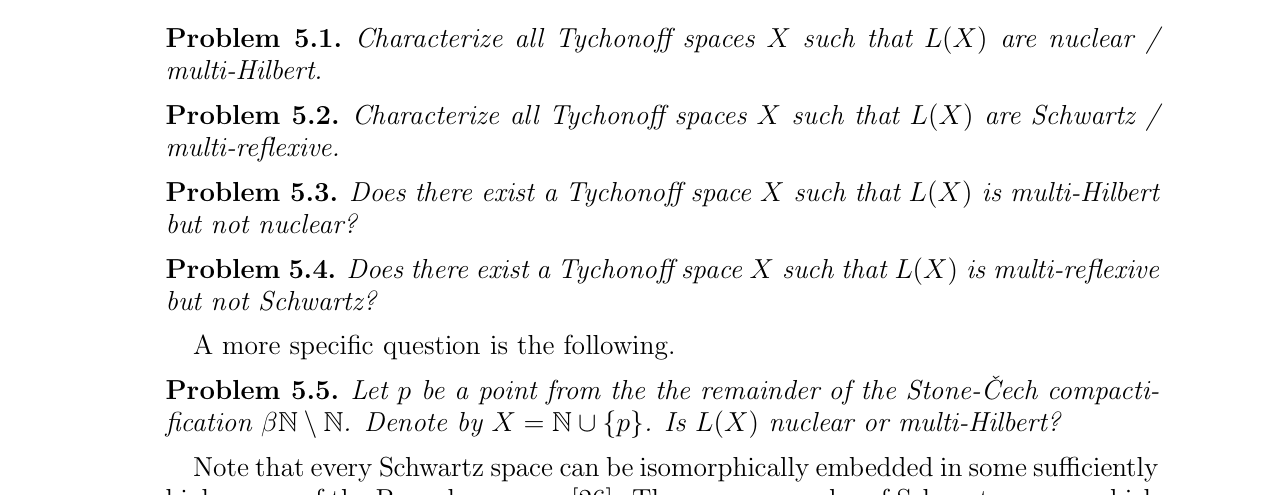
\includegraphics[width=\textwidth]{figures/open_problem_5_5_crop.png}
\end{center}

\section*{Definitions}

We identify \(p\in\beta\N\setminus\N\) with the corresponding free ultrafilter
on \(\N\). In the subspace \(X=\N\cup\{p\}\), each \(n\in\N\) is isolated and
the neighborhoods of \(p\) are exactly the sets \(\{p\}\cup A\), \(A\in p\).
For a scalar or normed-space-valued sequence \(z_n\), write \(z_n\to_p z\) if
\(\{n:z_n\in U\}\in p\) for every neighborhood \(U\) of \(z\).

An ultrafilter \(p\) is a \(P\)-point if every decreasing sequence
\((A_k)\subset p\) has a pseudointersection in \(p\), i.e. some \(A\in p\) with
\(A\setminus A_k\) finite for every \(k\). It is rapid if, for every increasing
\(m_k\), there is \(A=\{a_1<a_2<\cdots\}\in p\) such that \(a_k\ge m_k\) for
all sufficiently large \(k\).

We use the standard characterization of rapid ultrafilters by tall summable
ideals: for \(g:\N\to(0,\infty)\) with \(g(n)\to0\) and \(\sum_n g(n)=\infty\),
let
\[
   I_g=\left\{A\subset\N:\sum_{n\in A}g(n)<\infty\right\}.
\]
Then \(p\) is rapid iff \(p\cap I_g\ne\varnothing\) for every tall summable
ideal \(I_g\); see \cite[Theorem 1.1]{Flaskova}. The relevant theorem is
cropped here across the page break in \cite{Flaskova}.

\begin{center}
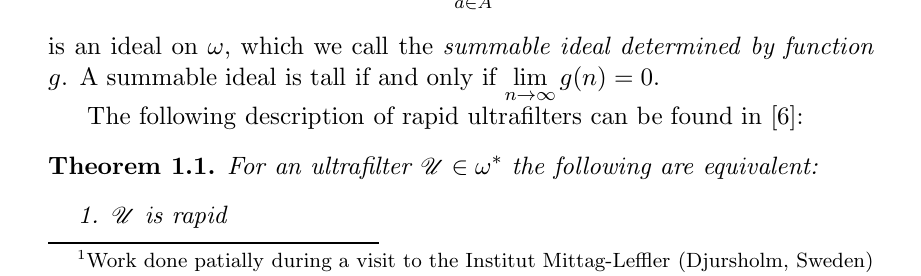
\includegraphics[width=.82\textwidth]{figures/rapid_summable_theorem_page1_crop.png}

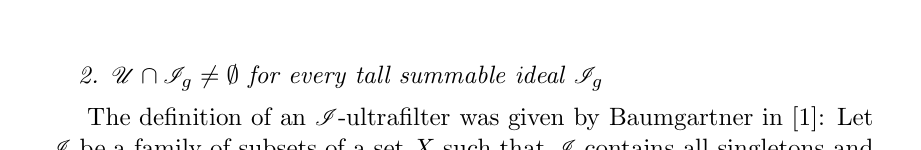
\includegraphics[width=.72\textwidth]{figures/rapid_summable_theorem_page2_crop.png}
\end{center}

\section*{Proof Intuition}

The topology of \(X\) turns continuous Banach-valued maps \(X\to E\) into
sequences in \(E\) that converge to the value at \(p\) along the ultrafilter.
Nuclearity asks whether every such sequence can be expanded by an absolutely
summable coordinate series whose scalar coordinate functions are uniformly
small near \(p\).

If \(p\) is both rapid and a \(P\)-point, the two set-theoretic properties
combine into exactly the diagonal selection needed: from every \(p\)-null norm
sequence one can choose a \(p\)-large subsequence on which the norms decay
superfast, and the remaining coordinates can be made harmless because they are
outside a \(p\)-large set. This gives a direct nuclear series for every Banach
map.

If either property fails, one can build a \(p\)-null scalar weight
\((\alpha_n)\) such that \(\sum_{n\in A}\alpha_n^2=\infty\) for every
\(A\in p\). The map \(n\mapsto \alpha_n e_n\) into \(\ell_1\) is then
continuous on \(X\), but any Hilbert factorization would put a \(p\)-large part
of these weighted coordinate vectors inside one ellipsoid in \(\ell_1\). A
simple adjoint/Rademacher-sign estimate says that this is possible only when
the corresponding square sum is finite, a contradiction.

\section*{Auxiliary Lemmas}

\begin{lemma}\label{lem:diagonal}
Let \(p\) be a rapid \(P\)-point and let \(a_n\ge0\) satisfy \(a_n\to_p0\).
Then there are positive numbers \(s_n\) such that \(s_n\to_p\infty\) and
\[
   \sum_{n=1}^{\infty}s_n a_n<\infty .
\]
\end{lemma}

\begin{proof}
Put \(B_k=\{n:a_n\le 2^{-k^2}\}\). After replacing \(B_k\) by
\(\bigcap_{j\le k}B_j\), assume \(B_{k+1}\subset B_k\); still \(B_k\in p\).
Since \(p\) is a \(P\)-point, choose \(C\in p\) such that \(C\setminus B_k\) is
finite for every \(k\). Choose increasing integers \(m_k\) so that
\[
   C\cap [m_k,\infty)\subset B_k .
\]
By rapidness, choose \(D=\{d_1<d_2<\cdots\}\in p\) with \(d_k\ge m_k\) for all
large \(k\). Let \(A=C\cap D=\{r_1<r_2<\cdots\}\in p\). Since \(A\subset D\),
we have \(r_k\ge d_k\), hence \(r_k\ge m_k\) eventually. Also \(r_k\in C\), so
\(r_k\in B_k\) eventually and therefore \(a_{r_k}\le2^{-k^2}\) eventually.

Set \(s_{r_k}=k\) for \(r_k\in A\). Enumerate \(\N\setminus A=\{t_j:j\ge1\}\)
and set \(s_{t_j}=2^{-j}(1+a_{t_j})^{-1}\). Then
\[
  \sum_{n\notin A}s_n a_n\le \sum_j2^{-j}<\infty,
  \qquad
  \sum_{k} s_{r_k}a_{r_k}\le\sum_k k2^{-k^2}+\text{finite}<\infty.
\]
Finally \(s_n\to_p\infty\), because \(A\in p\) and \(s_{r_k}=k\to\infty\) on
\(A\).
\end{proof}

\begin{lemma}\label{lem:equicont}
If \(s_n>0\) and \(s_n\to_p\infty\), then the functions
\[
   f_n=\frac{\chi_{\{n\}}}{s_n}\in C(X)
\]
form an equicontinuous pointwise bounded family on \(X\). Consequently their
linear extensions form an equicontinuous sequence in \(L(X)'\).
\end{lemma}

\begin{proof}
Pointwise boundedness is immediate: at \(m\in\N\) the supremum of
\(|f_n(m)|\) over \(n\) is \(1/s_m\), and at \(p\) it is \(0\). At an isolated
point there is no equicontinuity issue. At \(p\), given \(\varepsilon>0\), the
set \(A_\varepsilon=\{n:1/s_n<\varepsilon\}\) belongs to \(p\), and on
\(\{p\}\cup A_\varepsilon\) all functions \(f_n\) have absolute value
\(<\varepsilon\). The final assertion is the standard dual/equicontinuity
description for free locally convex spaces: equicontinuous pointwise bounded
families in \(C(X)\) extend to equicontinuous families of linear functionals on
\(L(X)\).
\end{proof}

\begin{lemma}\label{lem:ellipsoid}
Let \(T:H\to\ell_1\) be a bounded operator from a Hilbert space. If
\(\alpha_n e_n\in T(B_H)\) for all \(n\in A\), where \(B_H\) is the unit ball
and \(\alpha_n\ge0\), then
\[
   \sum_{n\in A}\alpha_n^2<\infty .
\]
\end{lemma}

\begin{proof}
Let \(\delta_n\) be the \(n\)-th coordinate functional on \(\ell_1\), and put
\(u_n=T^\ast\delta_n\in H\). For any finite \(F\subset A\) and any choice of
signs \(\varepsilon_n=\pm1\),
\[
   \left\|\sum_{n\in F}\varepsilon_n u_n\right\|
   =
   \left\|T^\ast\left(\sum_{n\in F}\varepsilon_n\delta_n\right)\right\|
   \le \|T\|,
\]
because \(\|\sum_{n\in F}\varepsilon_n\delta_n\|_{\ell_\infty}=1\). Averaging
the squared norm over all signs gives
\[
   \sum_{n\in F}\|u_n\|^2\le \|T\|^2.
\]
For each \(n\in A\), choose \(h_n\in B_H\) with \(T h_n=\alpha_n e_n\). Then
\[
   \alpha_n=\delta_n(T h_n)=\langle h_n,u_n\rangle\le \|u_n\|.
\]
Thus \(\sum_{n\in F}\alpha_n^2\le\|T\|^2\) for every finite \(F\subset A\),
which proves the claim.
\end{proof}

\begin{lemma}\label{lem:badweights}
If \(p\) is not a rapid \(P\)-point, then there are \(\alpha_n\ge0\) such that
\(\alpha_n\to_p0\) and
\[
   \sum_{n\in A}\alpha_n^2=\infty
   \quad\text{for every }A\in p.
\]
\end{lemma}

\begin{proof}
If \(p\) is not rapid, the summable-ideal characterization supplies a tall
summable ideal \(I_g\) with \(p\cap I_g=\varnothing\). Put
\(\alpha_n=\sqrt{g(n)}\). Then \(\alpha_n\to0\) ordinarily, hence
\(\alpha_n\to_p0\), and every \(A\in p\) has
\(\sum_{n\in A}\alpha_n^2=\sum_{n\in A}g(n)=\infty\).

It remains to handle the case in which \(p\) is rapid but not a \(P\)-point.
Choose a decreasing sequence \(P_k\in p\), with \(P_1=\N\), that has no
pseudointersection in \(p\). Let \(D_k=P_k\setminus P_{k+1}\), and define
\[
   \alpha_n^2=
   \begin{cases}
   1/k, & n\in D_k,\\
   0, & n\in \bigcap_k P_k.
   \end{cases}
\]
For every \(m\), \(P_m\subset\{n:\alpha_n^2\le 1/m\}\), so \(\alpha_n\to_p0\).
If some \(A\in p\) had \(\sum_{n\in A}\alpha_n^2<\infty\), then
\(A\cap D_k\) would be finite for every \(k\). Hence, for every \(m\),
\[
   A\setminus P_m\subset \bigcup_{k<m}(A\cap D_k)
\]
would be finite, making \(A\) a pseudointersection of \((P_k)\), a
contradiction.
\end{proof}

\section*{Main Theorem}

\begin{theorem}\label{thm:main}
Let \(p\in\beta\N\setminus\N\), let \(X=\N\cup\{p\}\), and let \(L(X)\) be the
free locally convex space over \(X\). The following are equivalent:
\begin{enumerate}[label=(\roman*)]
\item \(p\) is a rapid \(P\)-point;
\item \(L(X)\) is nuclear;
\item \(L(X)\) is multi-Hilbert.
\end{enumerate}
\end{theorem}

\begin{proof}
\((i)\Rightarrow(ii)\). Let \(T:L(X)\to E\) be a continuous linear map to a
Banach space. Write \(b=T(p)\) and \(x_n=T(n)-b\). Since \(T|_X\) is continuous
and \(f(p)=b\), the norm sequence \(a_n=\|x_n\|\) satisfies \(a_n\to_p0\).
By Lemma~\ref{lem:diagonal}, choose \(s_n>0\) with \(s_n\to_p\infty\) and
\(\sum_n s_n\|x_n\|<\infty\).

Let \(\sigma:L(X)\to\R\) be the continuous linear functional extending the
constant function \(1\) on \(X\). For \(x_n\ne0\), put
\[
   \lambda_n=s_n\|x_n\|,\qquad
   \varphi_n=\chi_{\{n\}}/s_n,\qquad
   y_n=x_n/\|x_n\|,
\]
and for \(x_n=0\) put \(\lambda_n=0\), \(y_n=0\), with the same
\(\varphi_n\). Then \(\sum_n|\lambda_n|<\infty\), the sequence \((y_n)\) is
bounded in \(E\), and \((\varphi_n)\) is equicontinuous in \(L(X)'\) by
Lemma~\ref{lem:equicont}. For every basis point of \(X\), and hence for every
element of \(L(X)\),
\[
   T(v)=\sigma(v)b+\sum_{n=1}^\infty \lambda_n\varphi_n(v)y_n .
\]
The first term is rank one and the series is nuclear. Thus every continuous
linear map from \(L(X)\) to a Banach space is nuclear, so \(L(X)\) is nuclear.

\((ii)\Rightarrow(iii)\). Every nuclear locally convex space is multi-Hilbert;
this is recalled in \cite[Section 2]{LU}.

\((iii)\Rightarrow(i)\). We prove the contrapositive. If \(p\) is not a rapid
\(P\)-point, choose \((\alpha_n)\) as in Lemma~\ref{lem:badweights}. Define
\(f:X\to\ell_1\) by \(f(p)=0\) and \(f(n)=\alpha_n e_n\). Since
\(\alpha_n\to_p0\), the map \(f\) is continuous and extends to a continuous
linear map \(\widehat f:L(X)\to\ell_1\).

Assume \(L(X)\) is multi-Hilbert. By the Hilbert-factorization lemma of
\cite[Lemma 2.4]{LU}, \(\widehat f\) factors as
\[
   L(X)\xrightarrow{S}H\xrightarrow{R}\ell_1
\]
with \(H\) Hilbert and \(R,S\) continuous linear. Let \(h_n=S(n)-S(p)\). Then
\(h_n\to_p0\), so \(A=\{n:\|h_n\|\le1\}\in p\). For \(n\in A\),
\[
   R h_n=\widehat f(n)-\widehat f(p)=\alpha_n e_n,
\]
so \(\{\alpha_n e_n:n\in A\}\subset R(B_H)\). Lemma~\ref{lem:ellipsoid}
implies \(\sum_{n\in A}\alpha_n^2<\infty\), contradicting the choice of
\((\alpha_n)\). Therefore \(L(X)\) is not multi-Hilbert.
\end{proof}

\begin{corollary}
If there are no rapid \(P\)-points in the ambient model of set theory, then
Problem 5.5 has the uniform negative answer: for every
\(p\in\beta\N\setminus\N\), \(L(\N\cup\{p\})\) is neither nuclear nor
multi-Hilbert. If \(p\) is a rapid \(P\)-point, then
\(L(\N\cup\{p\})\) is nuclear and hence multi-Hilbert.
\end{corollary}

\section*{Verification Notes}

The proof uses no numerical or computer-assisted step. The two technical
checks most worth human attention are:
\begin{itemize}
\item Lemma~\ref{lem:equicont}, where the standard free-LCS identification of
equicontinuous subsets of \(L(X)'\) with equicontinuous pointwise bounded
families in \(C(X)\) is invoked.
\item The positive implication, where the nuclear representation is checked on
the Hamel basis \(X\subset L(X)\); since all vectors in \(L(X)\) have finite
support in that basis, this determines the linear map.
\end{itemize}

\section*{Novelty and Literature Check}

Local run indexes were searched for \texttt{2106.13413}, \texttt{free locally
convex}, \texttt{multi-Hilbert}, \texttt{beta N}, \texttt{P-point}, and
\texttt{rapid ultrafilter}; no existing packet for this target was found. Web
searches on 2026-06-20 for exact and close phrases including
\texttt{"2106.13413" "Problem 5.5" "L(X)" nuclear},
\texttt{"N union \{p\}" "free locally convex" nuclear "multi-Hilbert"},
\texttt{"beta N" "free locally convex space" "multi-Hilbert"}, and
\texttt{"rapid P-point" "free locally convex" nuclear} did not locate a later paper
answering Problem 5.5. The proof uses the known rapid/summable-ideal
characterization recorded in \cite{Flaskova}; that paper is not an answer to
the free-LCS problem.

\section*{Human Review Recommendation}

Recommended for expert review as a likely full solution to Problem 5.5. The
result is concise but bridges free locally convex spaces and ultrafilter
combinatorics, so the main review should check the free-LCS equicontinuity
criterion and the rapid \(P\)-point diagonal lemma.

\begin{thebibliography}{9}

\bibitem{LU}
A. Leiderman and V. Uspenskij,
\emph{Is the free locally convex space \(L(X)\) nuclear?},
arXiv:2106.13413, 2021.
\url{https://arxiv.org/abs/2106.13413}

\bibitem{Flaskova}
J. Fla\v{s}kov\'a,
\emph{Rapid ultrafilters and summable ideals},
arXiv:1208.3690, 2012.
\url{https://arxiv.org/abs/1208.3690}

\end{thebibliography}

\end{document}
